%% Chapter 3 — Architecture with Explanation
%% Guideline target: 1–2 pages.
%%
%% This chapter should present the end-to-end system architecture — the
%% highest-level picture of what flows into what. One architecture diagram
%% is expected. Do NOT put implementation details here; that is Chapter 5.

\chapter{Architecture with Explanation}
\label{ch:architecture}

\section{System Overview}
\label{sec:arch-overview}

The proposed system follows a pipeline-based tooth-centric architecture that mimics the clinical diagnostic workflow. This process is broken down into multiple stages each responsible for a particular task. Instead of processing a single image for classification , the system decomposes it into individual tooth regions. The end-to-end pipeline consists of the following sequential stages: OPG input, image enhancement and normalization, tooth detection and FDI numbering, multi-disease detection, explainable AI, and structured report generation.

% Architecture figure — replace the placeholder with your diagram image.
\begin{figure}[htbp]
  \centering
   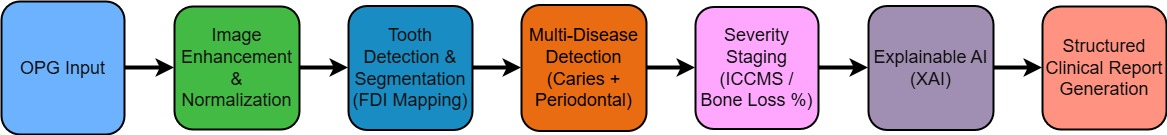
\includegraphics[width=0.9\linewidth]{fig1.jpeg}
  
  \caption{End-to-end system architecture.}
  \label{fig:architecture}
\end{figure}

\section{Component Description}
\label{sec:arch-components}


\subsection{OPG Input}
The first stage takes a panoramic radiograph as input. OPG images provide a complete view of the dentition and the surrounding structures, making them very useful for detecting multiple conditions. However, these images are often affected by low contrast, noise, and overlapping anatomical structures , which can make interpretation difficult. Due to these challenges, the raw image cannot be used directly for accurate analysis and requires preprocessing.

\subsection{Image Enhancement and Normalization}
The  image enhancement and normalization stage is required for improving the quality and consistency of the input data. Techniques such as contrast enhancement and intensity normalization are applied to bring out the subtle features that may help in detecting early-stage caries or slight variations in bone levels. Further, all images are resized and standardized to ensure compatibility with the deep learning models used in later stages. This step plays an important role in reducing variability across datasets and significantly improving the model’s performance .


\subsection{Tooth Detection and Segmentation}
Following the preprocessing, the system performs tooth detection and segmentation. A pretrained YOLO model trained on the dataset is used to process the full OPG image. It produces bounding box detections for each visible tooth. Then, these detections are mapped to standard FDI numbers (11-    48), allowing each tooth to be identified uniquely. These transformations allow to reduce noise by isolating each tooth, which helps in interpreting accurate results. This step is necessary for generating a clinically useful structured report at the later stage.



\subsection{Multi-Disease Detection}
In this stage the system performs multi-disease detection to identify both dental caries and periodontal disease detection within the same framework. For each tooth detected, two image crops are extracted, tightly cropped regions around the crown is passed to caries classification model and the larger expanded crop surrounding the alveolar bone region is passed to periodontal assessment model. This separation of analysis pathways improves accuracy and 
allows caries and bone loss to be evaluated from the same tooth bounding box .

\subsection{Severity Staging}
After detecting the presence of disease, the system performs severity staging to provide more clinically useful interpretations. For dental caries, severity is estimated based on the progression levels. For periodontal disease, bone loss percentage is calculated, which provides a quantitative measure of the disease progression. This stage is very critical as the detection alone is not enough for clinical decision making. BY including the severity grading, the system supports treatment planning.


\subsection{Explainable AI }
The system incorporates Grad-CAM explainability for providing visual explanations, which highlights the regions of the image that contributed to the model's prediction. These visual explanations allows clinicians to verify the reasoning behind the system's output are based on relevant features, enhancing transparency and trust.

\subsection{Structured Clinical Report Generation}
The final stage involves generating a structured clinical report. All predictions, including tooth-wise disease detection, severity classification, FDI tooth ID, and the corresponding Grad-CAM visualizations, are integrated into a final output. Instead of providing isolated predictions, the system provides a comprehensive summary that closely resembles a real diagnostic report.



\section{Design Rationale}
\label{sec:arch-rationale}

The tooth-centric decomposition approach was selected over other approaches like image-level classification, such as that used  by Bhoopalan et al. (2026), which achieved 96\% OPG-level accuracy using Vision Transformers (ViT). While effective at a global level, such approaches do not provide the per-tooth localization required for detailed clinical reporting. By focusing on individual teeth rather than the entire image,  the system improves interpretability and allows more precise predictions.

End-to-end transformer-based models were also taken into consideration but not adopted at this stage due to their high annotation requirements. Currently, there is no large-scale, multi-disease, multi-center public dataset of dental panoramic radiographs (OPGs) that supports such training. Additionally, their inference latency is approximately 40 seconds per image which makes them impractical for real-time clinical applications.

In contrast, a pipeline-based convolutional neural network (CNN) approach offers improved interpretability, modularity, and computational efficiency. Each component in the pipeline can be trained independently and updated as improved datasets or architectures become available. Explanability is also an important part of this design. Rather than treating the model as a black box, the system provides visual justifications for its predictions, making it more transparent and clinically more trustable.

